\begin{figure}[ht]
    \centering
    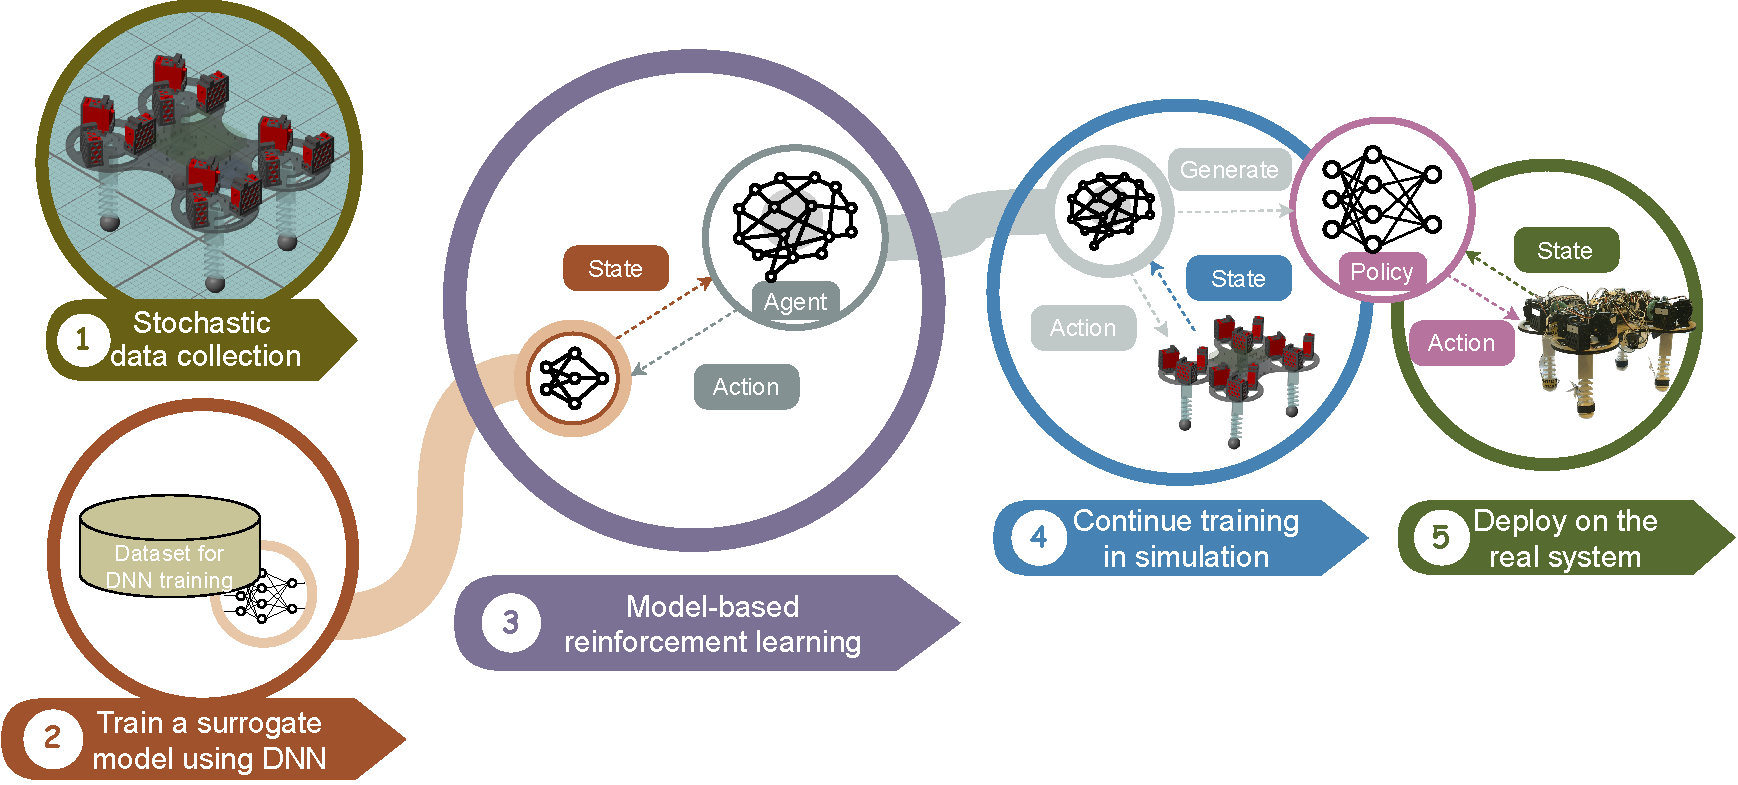
\includegraphics[width=\linewidth]{img/chap3/experiment.pdf}
    \caption{Creating a gait control policy. In the initial step, the physical parameters of the robot was identified and the stochastic actions were simulated in the identification to collect the data. In the subsequent step, an action-observation net was train that models complex robot model dynamics. The third step capitalized on the surrogate models produced in the previous two steps to train a control policy. In the fourth step, the trained control policy was further refined in simulation before deploying on the physical system.}
    \label{fig:exp}
\end{figure}

